\documentclass{article}
\usepackage[utf8]{inputenc}
\usepackage{graphicx}
\usepackage{listings}
\usepackage{float}
\usepackage{indentfirst}
\usepackage{xcolor}
\usepackage{hyperref}
\usepackage{fmtcount}
\usepackage{geometry}
\geometry{margin=1in}

\title{EEL 4712C - Digital Design: Lab Report 2}
\author{Cole Rottenberg \\ 11062528}
\date{February \ordinalnum{18}, 2024}

\lstset{
  language=VHDL,
  numbers=left,
  stepnumber=1,
  tabsize=2,
  numbersep=5pt,
  backgroundcolor=\color{white},
  showspaces=false,
  showtabs=true,
  frame=single,
  rulecolor=\color{black},
  captionpos=b,
  breaklines=true,
  breakatwhitespace=true,
  title=\lstname,
}

\begin{document}

\maketitle


\section*{Prelab Report}

\subsection*{Prelab Questions}
% Put all the answers to the prelab questions. These may be scanned using your phone or scanner. Not all prelabs have prelab questions
\subsubsection*{Demo:}
\begin{enumerate}
  \item Using the provided top\_level.vhd, the 7-segment display entity you created in Lab 0, and the provided fsm.vhdp synthesize your circuit.
  \item In Quartus, assign pins to the inputs (switches \& buttons) and outputs (LEDs) such that the correct outputs are displayed on the 7-segment display.
  \item Show your TA the RTL viewer showing the properly synthesized datapath.
  \item Once the everything is working, show a TA the correct output for Fib(11) = 89.
\end{enumerate}

\subsection*{Prelab Design and Implementation}
% Go into detail about how you designed any design parts of the prelab. Then, go into detail about how you implemented any implementation parts of the prelab
The prelab for this lab required the implementation of a fibonacci calculator datapath. The datapath was to be implemented using a combinations of multiplexers, adders, and registers. Then, the design of the datapath was implemented in VHDL. The design was then tested by flashing the FPGA with the design and testing the output of the design. The following is the implementation of the datapath is in the Appendix under Listing \ref{lst:datapath-vhdl-code}.

\subsection*{Reflection}
% Talk about what you learned during the prelab. Bring up anything that was a stumped you for a while. Bring up any accomplishments you were proud of.
During the prelab, I learned the importantance of READING the entire lab manual before starting the prelab. I ended up implementing my own fibonacci logic in a single VHDL file. I wasted a good amount of time doing this, and I could have saved time by reading the lab manual. I was proud of my ability to implement the fibonacci logic in VHDL, but I was disappointed that I wasted time doing so.

\section*{Postlab Report}

\subsection*{Problem Statement}
% Provide a short informal description of the lab’s goals (From the lab assignment)
% If required, specify the system to design.
% - Define the inputs.
% - Define the outputs.
% - Define the function of your system. 
% This section should be 1-2 paragraphs long.
The objective of this lab is to design a datapath capable of calculating the Nth Fibonacci
number along with a testbench to verify its correctness. The algorithm for computing the
Nth Fibonacci number is shown below; make sure you read and understand this code
before continuing on to writing the datapath or testbench. The inputs to the datapath are a reset, a clock, and the input N, and a go signal. The output of the datapath is the Nth Fibonacci number. The function of the system is to calculate the Nth Fibonacci number.

\subsection*{Design}
% Describe the design decisions you made.
% - What components did you use?
The design followed a given schematic that involved the use of multiplexers, adders, comparators, and registers. These components were then interconnected to form the fibonacci datapath. The signals that connected these units were primarily std\_logic\_vectors that were 24 bits wide. The algorithm used was based on starts at 2 and understanding that the first two numbers in the fibonacci sequence are 0 and 1. We also implemented essentially a for loop within VHDL 
% - What signals did you use to connect the components?
% - What algorithms did you use?
% Code Segment or block diagrams may be included here.
% Explain your design choices(pros/cons).
% Any designs made in prelab should be included here but more briefly.
% This section should be 1-2 paragraphs long.

\subsection*{Implementation}
% Describe the implementation process.
% Code segments or block diagrams may be included here.
% What time did you need to complete your design?
% This section should be 1-2 paragraphs long.
The implementation of the design can be found in the Appendix under Listing \ref{lst:datapath-vhdl-code}. For individual components, the implementation was relatively straightforward. The mux can be seen in Listing \ref{lst:mux-vhdl-code}, the adder in Listing \ref{lst:add-vhdl-code}, the register in Listing \ref{lst:reg-vhdl-code}, and the comparator in Listing \ref{lst:comparator-vhdl-code}. The implementation of the datapath was more complex, but it was still relatively straightforward. The implementation of the datapath was completed in a few hours. 

\subsection*{Testing}
% Describe how you tested your design.
% Did everything work as expected?
% - Did inputs match the expected outputs?
% - Special cases?
% Include if possible, timing diagram of photo/video of the system.
Testing the design was relatively straightforward. After working past syntax errors, the design was able to compile and after assigning the correct outputs to LEDs, the code worked immeadiately. The design was also tested in ModelSim with 11 as the input, and the output was 89, which is the correct output for the 11th number in the fibonacci sequence. In figure \ref{fig:model-sim}, the ModelSim simulation of the datapath can be seen. The simulation shows the correct output for the 11th number in the fibonacci sequence. The design was also tested on the FPGA board, and the output was 89, which is the correct output for the 11th number in the fibonacci sequence. The FPGA board with the working datapath can be seen in figure \ref{fig:fpga-demo}.

NOTE: Testing in ModelSim was done before the datapath redesign and was tested with my own fibonacci logic which is similar to the given logic. The given logic was tested on the FPGA board and worked as expected.

\subsection*{Conclusions}
% Summarize in one paragraph, the work you did, the success and problems you encountered, and how to improve next in the future.
% This section should only be 1 paragraph long.
The work in this lab was incredibly foundational considering the practice of structural architecture and use of multiple components to create a single, complex system. The lab was successful in that the design was able to be implemented and tested on the FPGA board. The only problem encountered was the time wasted in the prelab. In the future, I will be sure to read the entire lab manual before starting the prelab.

\section*{Appendix}
% Include all postlab code, screenshots, and simulations here. ALL SIMULATIONS MUST BE ANNOTATED. This means pointing out particularly important parts of a simulation. This can be done with arrows or textboxes. All figures must be captioned. Code should be commented a fair amount.

% Figure of ModelSim simulation
\begin{figure}[H]
  \centering
  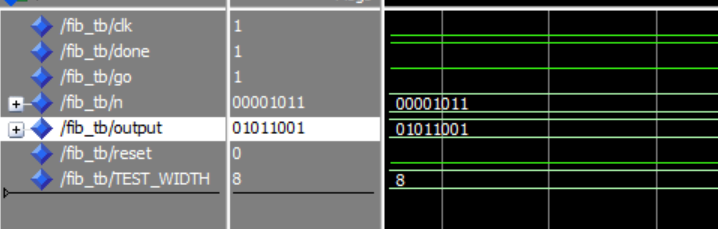
\includegraphics[width=0.8\textwidth]{P1_sim/fib_tb_sim.png}
  \caption{ModelSim Simulation of Datapath}
  \label{fig:model-sim}
\end{figure}

% Demo of working FPGA board
\begin{figure}[H]
  \centering
  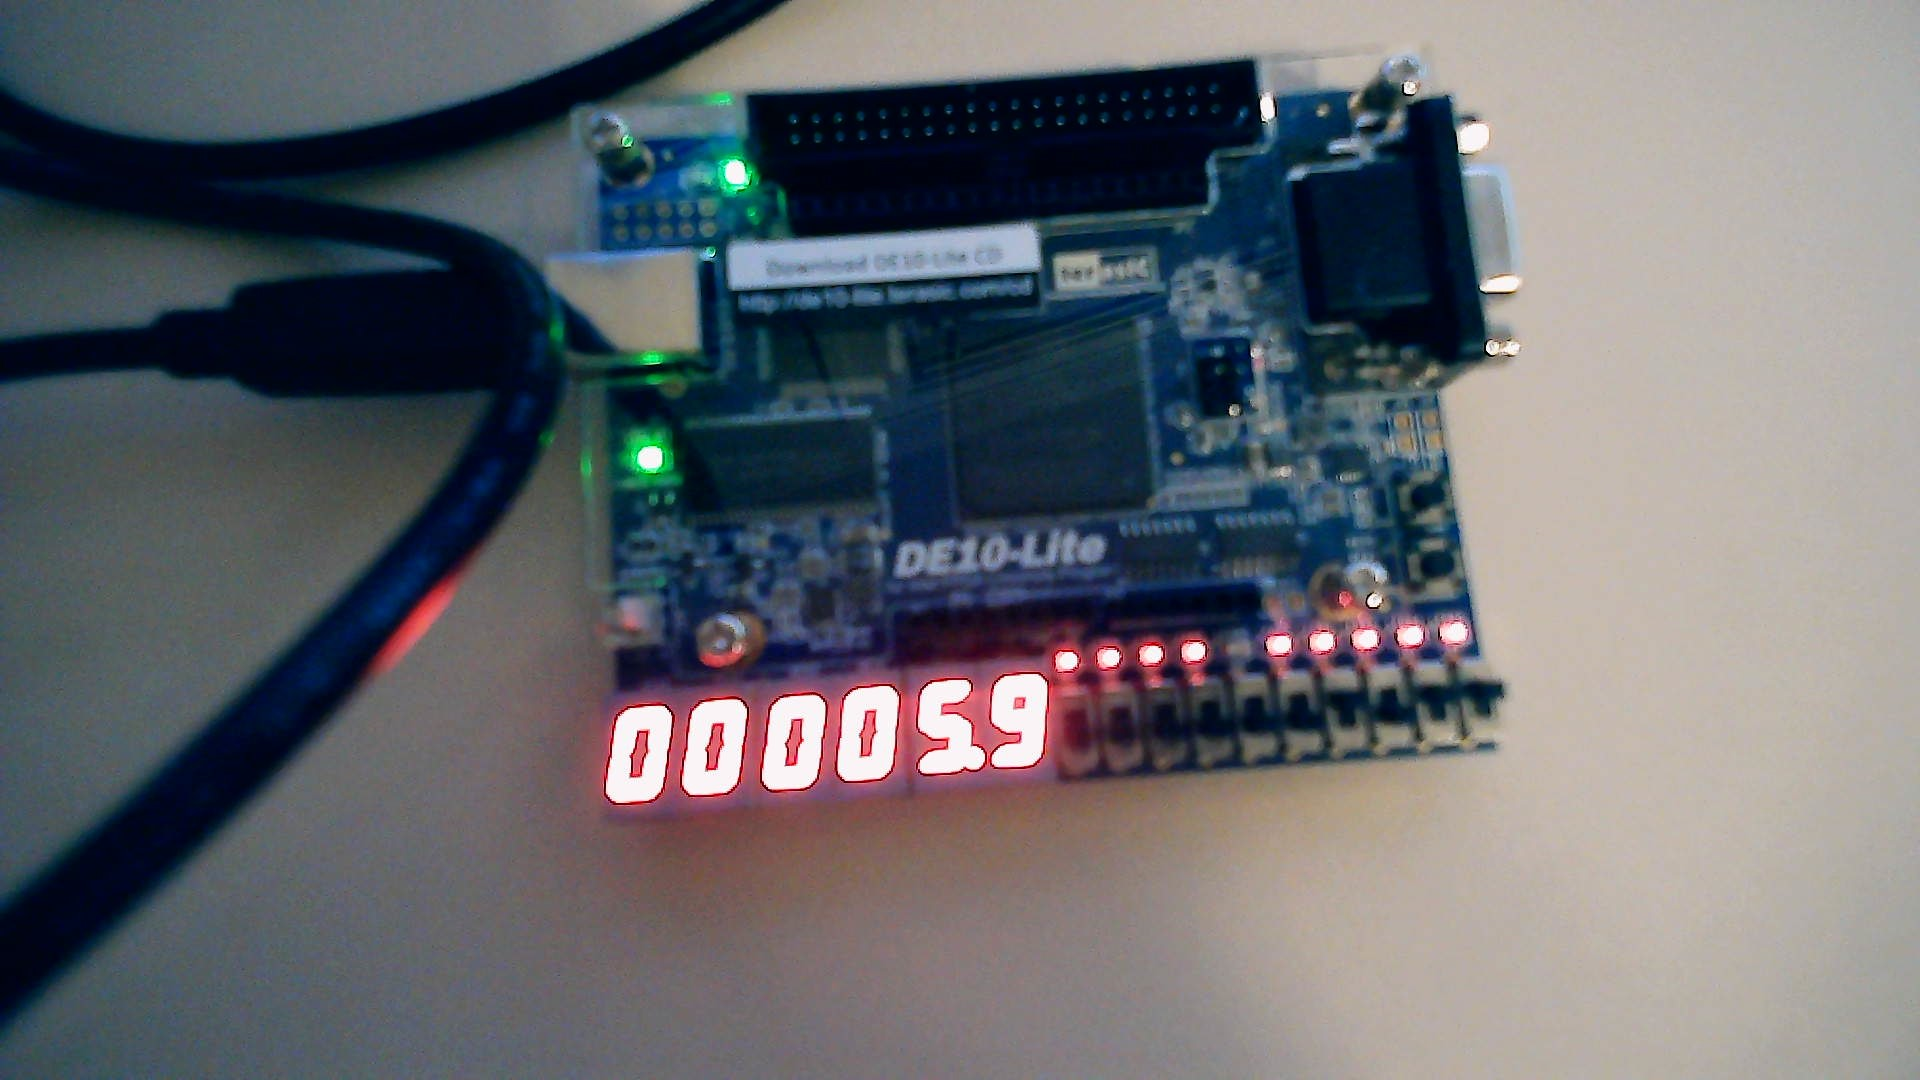
\includegraphics[width=0.8\textwidth]{Fib11_Demo.jpg}
  \caption{FPGA Board with Working Datapath}
  \label{fig:fpga-demo}
\end{figure}

\begin{lstlisting}[caption=Datapath VHDL Code, label=lst:datapath-vhdl-code]
library ieee;
use ieee.std_logic_1164.all;
use ieee.numeric_std.all;

-- Datapath for fibonacci sequence

entity datapath is
    generic(
      width : integer := 24
    );
    port(
      -- clk and rst
      clk: in std_logic;
      rst : in std_logic;
      
      -- i/o 
      n : in std_logic_vector(5 downto 0);
      result : out std_logic_vector(23 downto 0);
      -- control inputs
      x_sel : in std_logic;
      y_sel : in std_logic;
      i_sel : in std_logic;
      result_sel : in std_logic;


      n_en : in std_logic;
      result_en : in std_logic;
      x_en : in std_logic;
      y_en : in std_logic;
      i_en : in std_logic;
      n_eq_0 : out std_logic;

      -- status signals
      i_le_n : out std_logic
    );
end datapath;

-- The datapath is composed of registers, fibonacci logic and other components

-- The datapath starts with a register for the input n
-- if n_en is high, the input n is loaded into the register
-- afterwards, the register is connected to the fibonacci logic

architecture rtl of datapath is
    signal i_reg_out, x_reg_out, y_reg_out, n_reg_out : std_logic_vector(width-1 downto 0);
    signal i_mux_out, x_mux_out, y_mux_out, result_mux_out : std_logic_vector(width-1 downto 0);
    signal add1_out, add2_out : std_logic_vector(width-1 downto 0);
    signal n_scaled : std_logic_vector(width-1 downto 0);
  -- Build input register and logic 
    begin
  
  -- Connecting components to impl fibonacci logic using registers,mux, adders and comparators
        I_MUX : entity work.mux
            generic map(
                width => width
            )
            port map(
                input1 => add1_out,
                input2 => std_logic_vector(to_unsigned(2, width)),
                sel => i_sel,
                output => i_mux_out
            );
    
        X_MUX : entity work.mux
            generic map(
                width => width
            )
            port map(
                input1 => y_reg_out,
                input2 => std_logic_vector(to_unsigned(0, width)),
                sel => x_sel,
                output => x_mux_out
            );

        Y_MUX : entity work.mux
            generic map(
                width => width
            )
            port map(
                input1 => add2_out,
                input2 => std_logic_vector(to_unsigned(1, width)),
                sel => y_sel,
                output => y_mux_out
            );

        RESULT_MUX : entity work.mux
            generic map(
                width => width
            )
            port map(
                input1 => y_reg_out,
                input2 => std_logic_vector(to_unsigned(0, width)),
                sel => result_sel,
                output => result
            );

        -- REGISTERS

        I_REG : entity work.reg
            generic map(
                width => width
            )
            port map(
                clk => clk,
                reset => rst,
                d => i_mux_out,
                q => i_reg_out,
                en => i_en
            );

        X_REG : entity work.reg
            generic map(
                width => width
            )
            port map(
                clk => clk,
                reset => rst,
                d => x_mux_out,
                q => x_reg_out,
                en => x_en
            );

        Y_REG : entity work.reg
            generic map(
                width => width
            )
            port map(
                clk => clk,
                reset => rst,
                d => y_mux_out,
                q => y_reg_out,
                en => y_en
            );

        N_REG : entity work.reg
            generic map(
                width => width
            )
            port map(
                clk => clk,
                reset => rst,
                d => (width-1-6 downto 0 => '0') & n,
                q => n_reg_out,
                en => n_en
            );

        -- ADDERS

        ADD1 : entity work.add
            generic map(
                width => width
            )
            port map(
                in1 => std_logic_vector(to_unsigned(1, width)),
                in2 => i_reg_out,
                output => add1_out
            );

        ADD2 : entity work.add
            generic map(
                width => width
            )
            port map(
                in1 => x_reg_out,
                in2 => y_reg_out,
                output => add2_out
            );

        -- COMPARATOR
        N_COMP : entity work.comparator
            generic map(
                width => width
            )
            port map(
                a => n_reg_out,
                b => std_logic_vector(to_unsigned(0, width)),
                eq => n_eq_0
            );
        
        LE_COMP : entity work.comparator
            generic map(
                width => width
            )
            port map(
                a => i_reg_out,
                b => n_reg_out,
                le => i_le_n
            );
end rtl;
\end{lstlisting}

% Begin Mux, add, reg, and comparator VHDL code

\begin{lstlisting}[caption=Mux VHDL Code, label=lst:mux-vhdl-code]
library ieee;
use ieee.std_logic_1164.all;
use ieee.std_logic_arith.all;
use ieee.numeric_std.all;

entity mux is 
    generic(
        width : integer := 6
    );
    port(
        input1 : in std_logic_vector(width-1 downto 0);
        input2 : in std_logic_vector(width-1 downto 0);
        sel : in std_logic;
        output : out std_logic_vector(width-1 downto 0)
    );

end entity mux;

architecture rtl of mux is
begin
    process(input1, input2, sel)
    begin
        if sel = '0' then
            output <= input1;
        else
            output <= input2;
        end if;
    end process;
end architecture rtl;
\end{lstlisting}

\begin{lstlisting}[caption=Add VHDL Code, label=lst:add-vhdl-code]
library ieee;
use ieee.std_logic_1164.all;
use ieee.numeric_std.all;
-- Adder entity
entity add is 
    generic(width: integer := 6);
    port(
        in1 : in std_logic_vector(width-1 downto 0);
        in2 : in std_logic_vector(width-1 downto 0);
        output : out std_logic_vector(width-1 downto 0)
    );
end add;

-- Adder architecture
architecture arch of add is
begin
    output <= std_logic_vector(unsigned(in1) + unsigned(in2));
end arch;
\end{lstlisting}

\begin{lstlisting}[caption=Reg VHDL Code, label=lst:reg-vhdl-code]
library ieee;
use ieee.std_logic_1164.all;
use ieee.numeric_std.all;
entity reg is
    generic(
	 width : integer := 6
	 );
    port(
        clk: in std_logic;
        reset: in std_logic;
        d: in std_logic_vector(width-1 downto 0);
        q: out std_logic_vector(width-1 downto 0);
        en : in std_logic
    );
end entity;

architecture rtl of reg is
begin
    process(clk, reset)
    begin
        if reset = '1' then
            q <= (others => '0');
        elsif rising_edge(clk) then
            if en = '1' then
                q <= d;
            end if;
        end if;
    end process;
end rtl;
\end{lstlisting}

\begin{lstlisting}[caption=Comparator VHDL Code, label=lst:comparator-vhdl-code]
library ieee;
use ieee.std_logic_1164.all;
use ieee.numeric_std.all;

-- Comparator entity
entity comparator is
    generic(width : integer := 6);
    port (
        a : in std_logic_vector(width-1 downto 0);
        b : in std_logic_vector(width-1 downto 0);
        le : out std_logic;
        eq : out std_logic
    );
end comparator;

-- Comparator architecture

architecture behavioral of comparator is
    begin
        process(a,b)
        begin 
        -- Less than or equal to
        if (unsigned(a) <= unsigned(b)) then
            le <= '1';
        else
            le <= '0';
        end if;
        -- Equal to
        if (unsigned(a) = unsigned(b)) then
            eq <= '1';
        else
            eq <= '0';
        end if;
        end process;
end behavioral;
\end{lstlisting}
\end{document}
